
%%% Local Variables:
%%% mode: latex
%%% TeX-master: "os-book-pt_BR"
%%% End:

\def\dx{3cm}
\def\dy{2cm}
\colorlet{kernel color}{black!80}
\colorlet{user color}{blue!40!black}

\begin{figure}
 \centering
 % COLORS	

  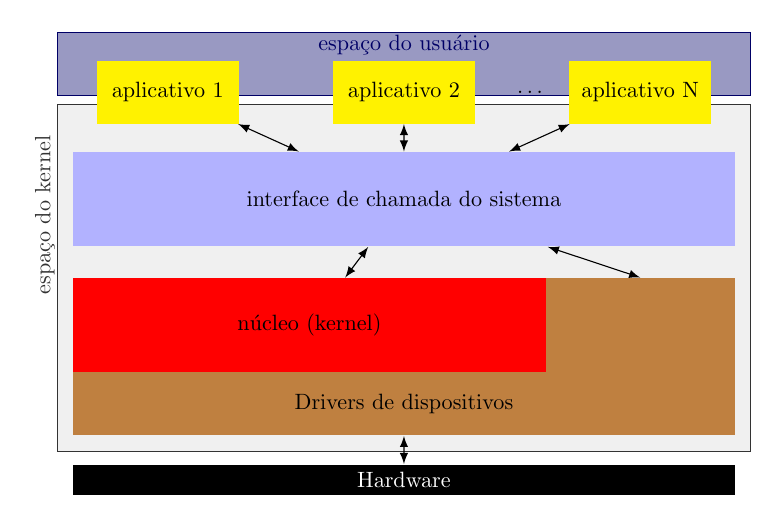
\begin{tikzpicture}[scale=.8,
    every node/.style={transform shape},
    application/.style={fill=yellow,minimum height=.5*\dy,minimum
      width=.75*\dx}
    ]

    \node[color=white,fill=black,minimum width=3.5*\dx] (hardware) {Hardware};

    \node<6->[minimum width=11cm,minimum height=5.5cm,anchor=south,fill opacity=.4,fill=gray!30,draw=kernel color] (kernel space) 
    [above of=hardware,yshift=1.1*\dy] {};
    \node<6->[color=kernel color,rotate=90] [right of=kernel space,yshift=2.85*\dy] {espaço do kernel};

    \node<7->[minimum width=11cm,minimum height=1cm,anchor=south,fill opacity=.4,fill=user color,draw=user color] (user space) 
    [above of=kernel space,yshift=1.2*\dy] {};
    \node<7->[color=user color] [above of=user space,yshift=-.35*\dy] {espaço do usuário};

    \node<2->[fill=brown,minimum height=.5*\dy,minimum width=3.5*\dx] (device driver) [above of=hardware,yshift=.1*\dy] {Drivers de dispositivos};
    \node<2->[fill=brown,minimum height=1*\dy,minimum width=\dx] (top device driver) [above of=device driver,xshift=1.25*\dx] {};
    \node<3->[fill=red,minimum height=.75*\dy,minimum width=2.5*\dx] (kernel) [above of=device driver,xshift=-.5*\dx,yshift=.125*\dy] {núcleo (kernel)};
    \node<4->[fill=blue!30,minimum height=.75*\dy,minimum width=3.5*\dx] (system call) 
    [above of=kernel,xshift=.5*\dx,yshift=.5*\dy] {interface de chamada do sistema};

    \node<5->[application] (app2) [above of=system call, yshift=.35*\dy] {aplicativo 2};
    \node<5->[application] (app1) [left of=app2,xshift=-2.75cm] {aplicativo 1};
    \node<5->[application] (appn) [right of=app2,xshift=2.75cm] {aplicativo N};
    \node<5->[right of=app2,xshift=1cm] {$\dots$};

    \draw<2->[<->,>=latex] (device driver) -- (hardware);
    \draw<4->[<->,>=latex] (kernel) -- (system call);
    \draw<4->[<->,>=latex] (top device driver.north) -- (system call);
    \draw<5->[<->,>=latex] (app1) -- (system call);
    \draw<5->[<->,>=latex] (app2) -- (system call);
    \draw<5->[<->,>=latex] (appn) -- (system call);

  \end{tikzpicture}

\label{fig:00intro:monokernel}
\caption{Arquitetura tradicional de um kernel monolítico.}

\end{figure}
